% Created 2016-03-16 Wed 09:37
\documentclass[bigger]{beamer}
\usepackage[utf8]{inputenc}
\usepackage[T1]{fontenc}
\usepackage{fixltx2e}
\usepackage{graphicx}
\usepackage{longtable}
\usepackage{float}
\usepackage{wrapfig}
\usepackage{rotating}
\usepackage[normalem]{ulem}
\usepackage{amsmath}
\usepackage{textcomp}
\usepackage{marvosym}
\usepackage{wasysym}
\usepackage{amssymb}
\usepackage{hyperref}
\tolerance=1000
\usetheme{default}
\author{Weston Dransfield}
\date{\today}
\title{Completeness: 3COLOR}
\hypersetup{
  pdfkeywords={},
  pdfsubject={},
  pdfcreator={Emacs 24.5.1 (Org mode 8.2.10)}}
\begin{document}

\maketitle
\begin{frame}{Outline}
\tableofcontents
\end{frame}


\begin{frame}[label=sec-1]{Description}
\textbf{\textit{3COLOR}} = \{\(\langle G \rangle\) | the nodes of G can be colored with three colors such that no two adjacent nodes are the same color \}
\end{frame}

\begin{frame}[label=sec-2]{Example}
\begin{center}
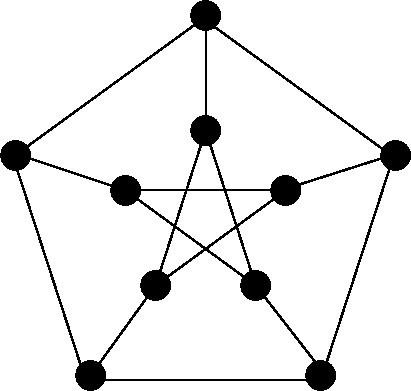
\includegraphics[width=7cm]{uncolored.jpg}
\end{center}
\end{frame}

\begin{frame}[label=sec-3]{Example}
\begin{center}
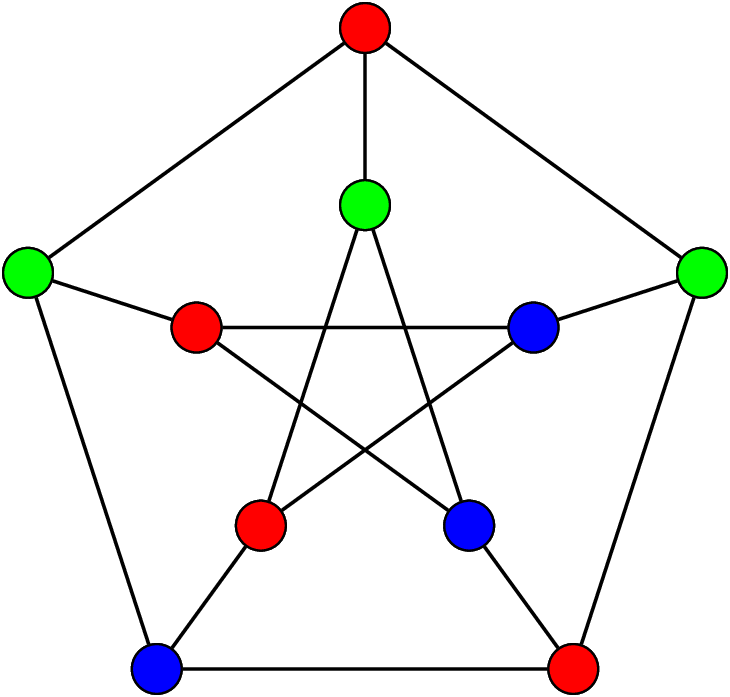
\includegraphics[width=7cm]{colored.png}
\end{center}
\end{frame}


\begin{frame}[label=sec-4]{The Problem}
Is a given graph \(G\) a member of \textbf{\textit{3COLOR}}?

\begin{itemize}
\item<2-> This is tough to decide, but easy to verify!
\end{itemize}
\end{frame}

\begin{frame}[label=sec-5]{The Verifier}
\(V\) = "On input \(\langle G, c \rangle\),
\begin{enumerate}
\item<1-> Check that c includes 3 colors.
\item<2-> Color each node of G as specified by c.
\item<3-> For each node, check that each adjacent node is not the same color.
\item<4-> If all checks pass accept, otherwise reject."
\end{enumerate}

\begin{itemize}
\item<5->Step 3 has largest time complexity of \(O(n^2)\). 3COLOR is in NP because it can be verified in polynomial time.
\end{itemize}
\end{frame}


\begin{frame}[label=sec-6]{Constructing the Reduction}
Construct a transformation \(T\) from \(3SAT\) to \(3COLOR\).
\begin{enumerate}
\item<2-> Establish Truthiness
\item<3-> Force variables to be true or false
\item<4-> Use these subgraphs to create a graph that is 3 colorable iff the statement is satisfiable
\end{enumerate}
\end{frame}

\begin{frame}[label=sec-7]{Constructing the Reduction - Truthiness}
\begin{center}
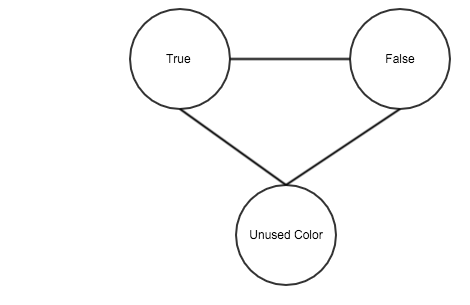
\includegraphics[width=7cm]{Truthiness.png}
\end{center}
\end{frame}

\begin{frame}[label=sec-8]{Constructing the Reduction - Variables}
\begin{center}
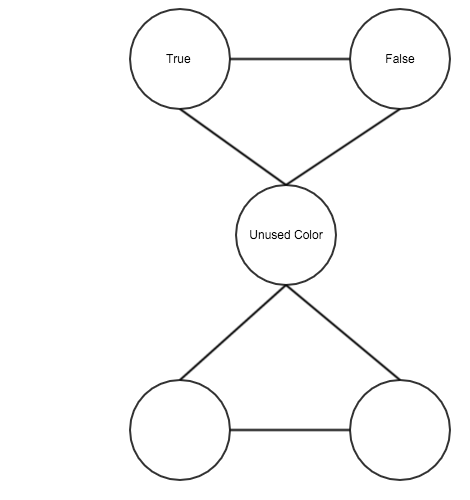
\includegraphics[width=7cm]{Variable1.png}
\end{center}
\end{frame}

\begin{frame}[label=sec-9]{Constructing the Reduction - Variables}
\begin{center}
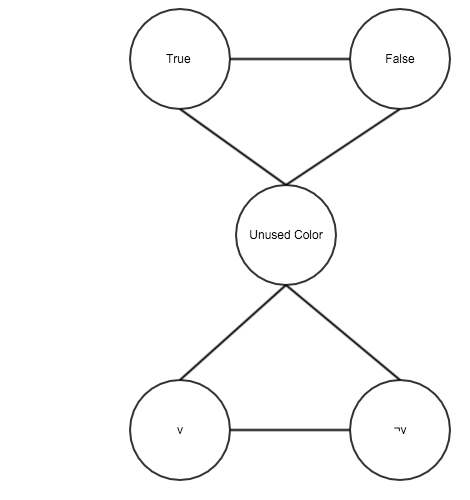
\includegraphics[width=7cm]{Variable2.png}
\end{center}
\end{frame}

\begin{frame}[label=sec-10]{Constructing the Reduction - OR}
\begin{center}
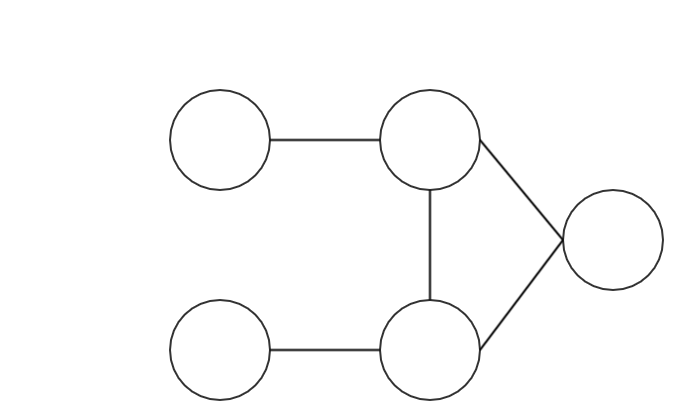
\includegraphics[width=7cm]{Or1.png}
\end{center}

Output node is colored false if both input nodes are colored false
\begin{itemize}
\item <1-> Need to attach to truthiness gadget
\end{itemize}
\end{frame}

\begin{frame}[label=sec-11]{Constructing the Reduction - OR}
\begin{center}
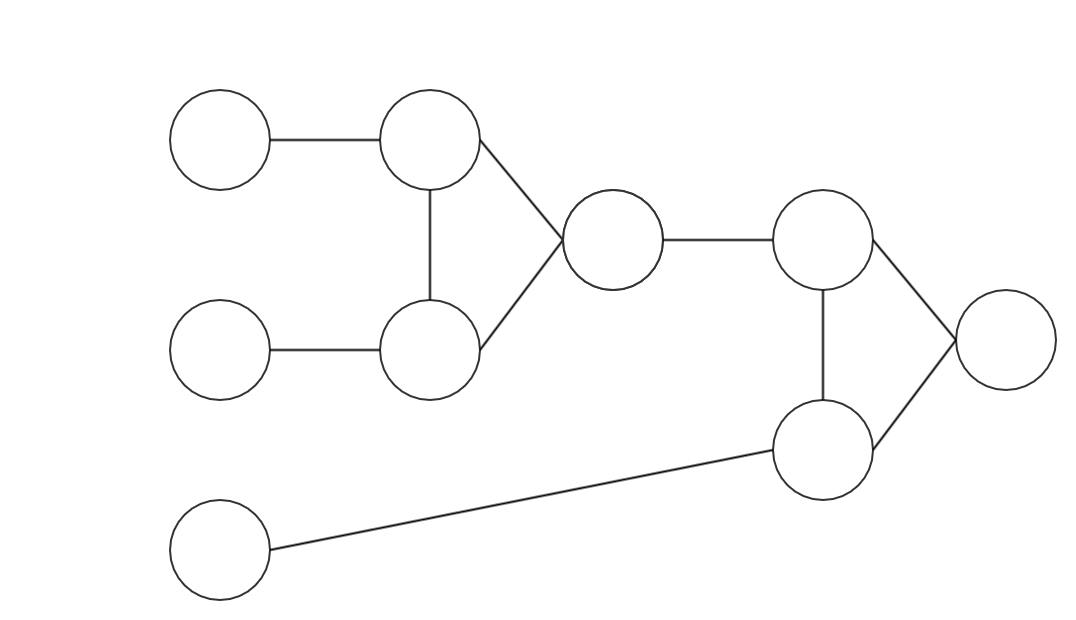
\includegraphics[width=10cm]{Or2.png}
\end{center}
\end{frame}

\begin{frame}[label=sec-12]{Constructing the Reduction - Clause}
\begin{center}
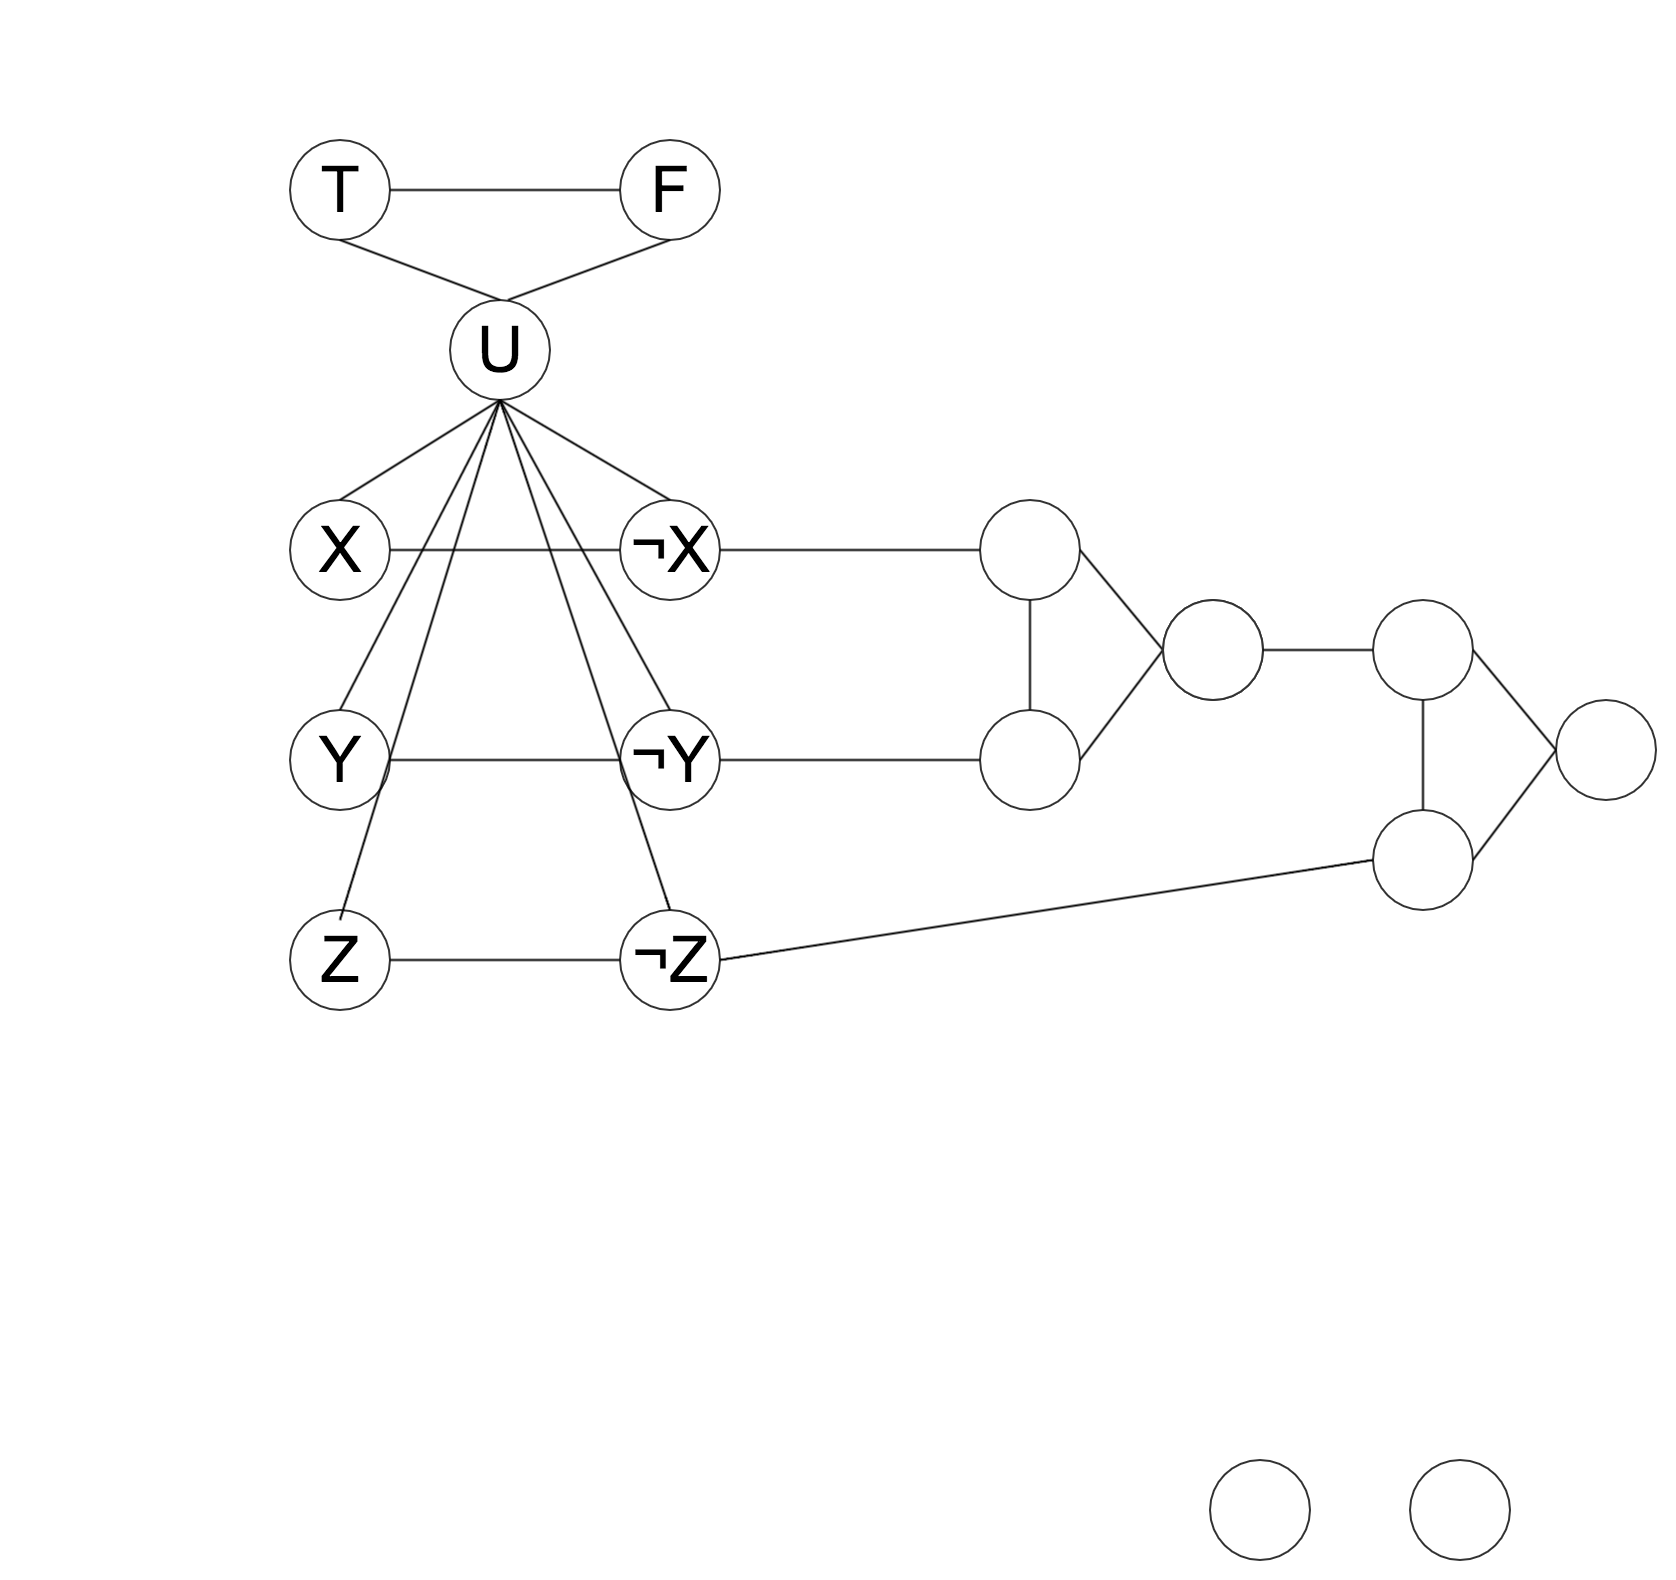
\includegraphics[width=10cm]{Comb1.png}
\end{center}
\end{frame}

\begin{frame}[label=sec-13]{Constructing the Reduction - Clause}
\begin{center}
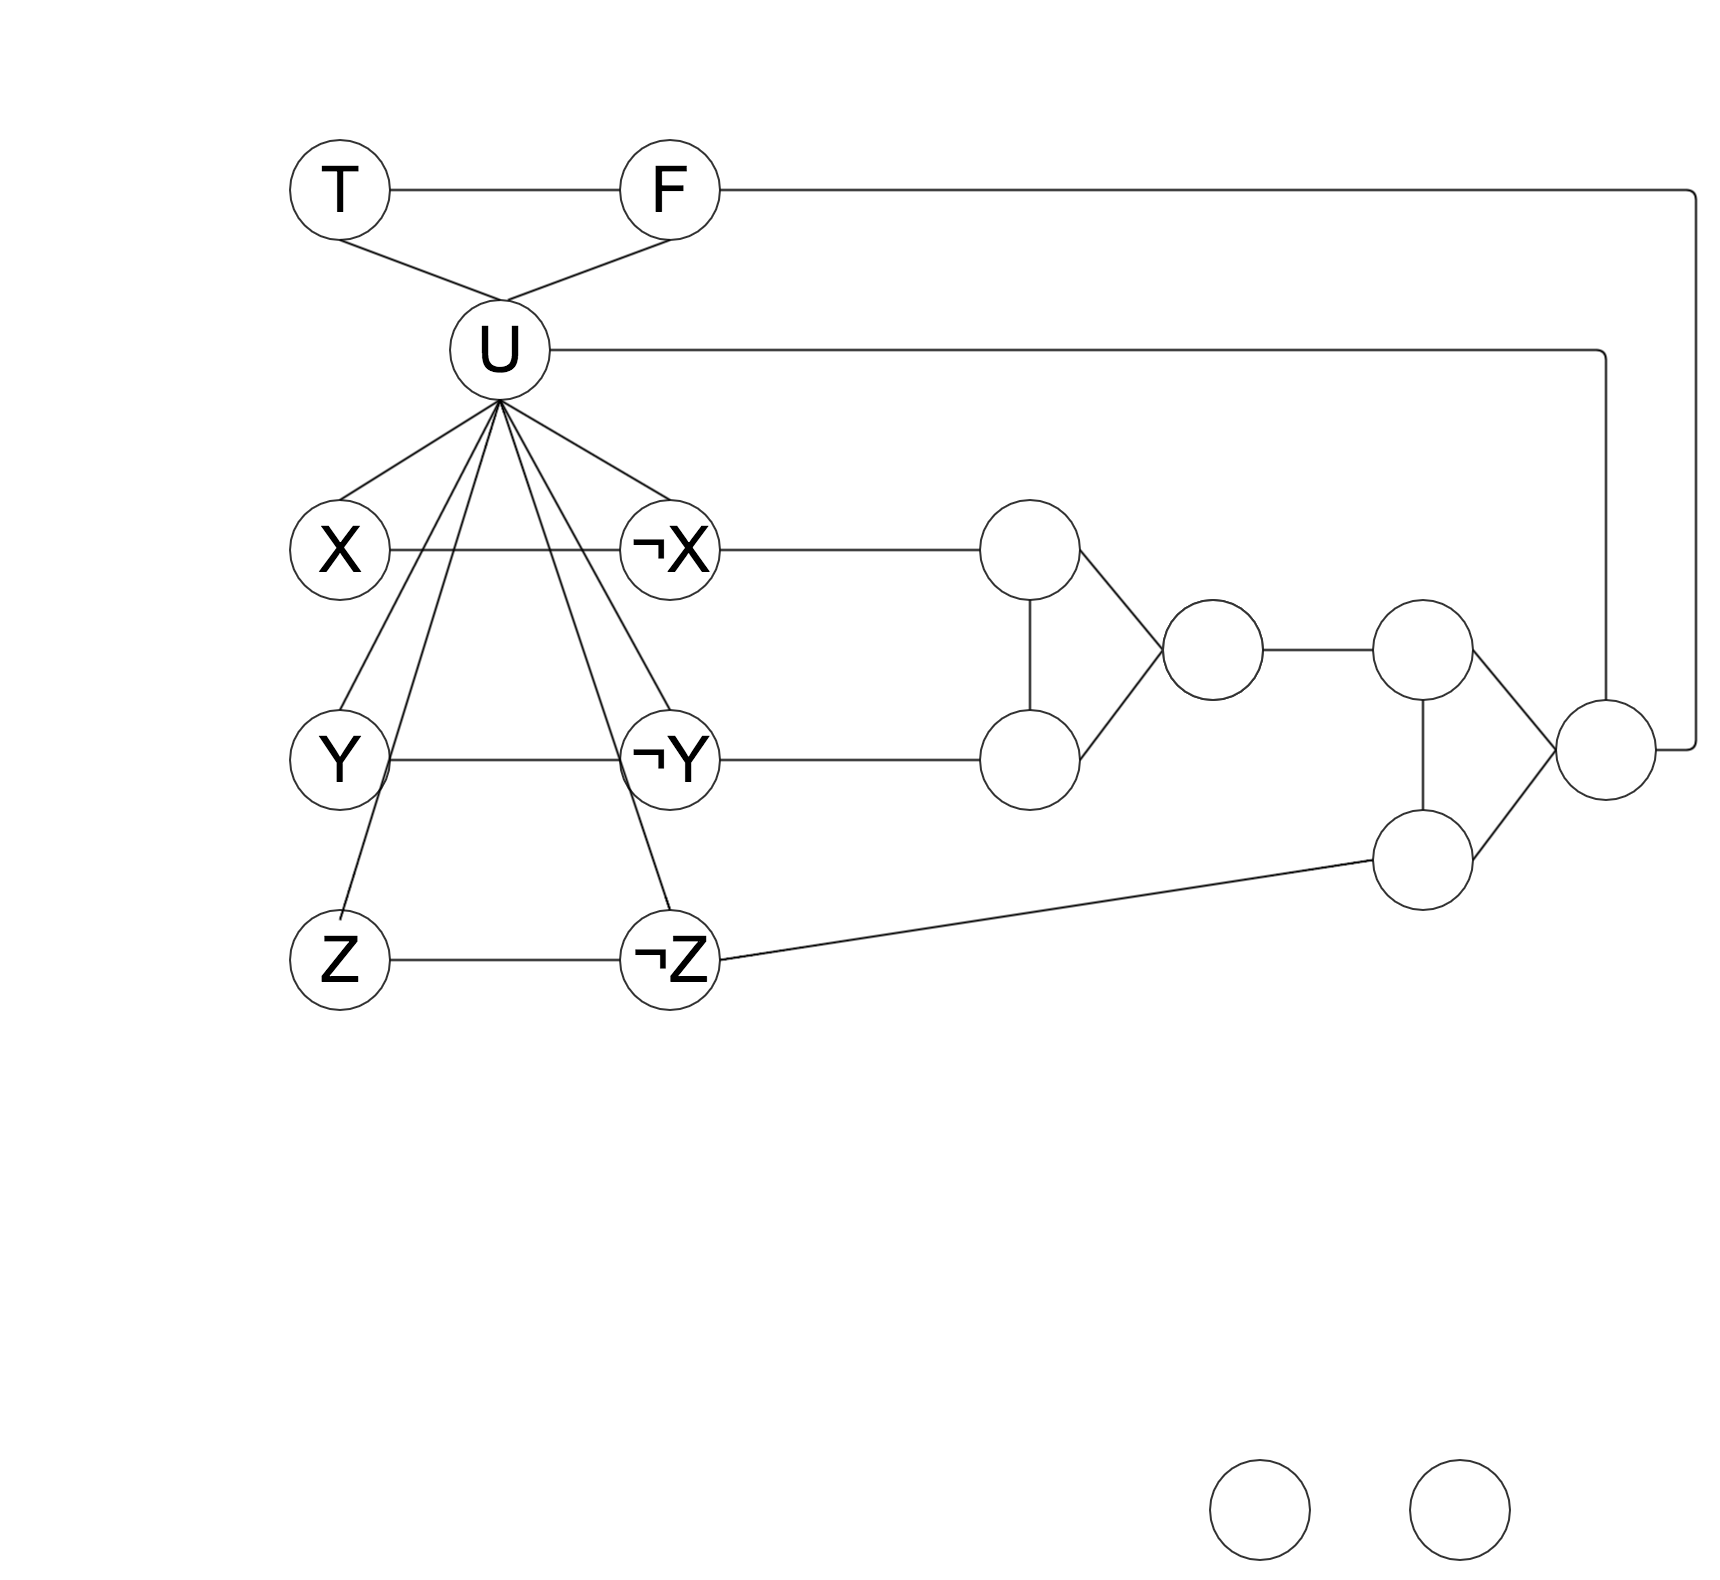
\includegraphics[width=10cm]{Comb2.png}
\end{center}
\end{frame}

\begin{frame}[label=sec-14]{}
\begin{center}

\includegraphics[width=12cm]{bats.png}
\end{center}
\end{frame}

\begin{frame}[label=sec-15]{Transformation}
Transform expression \(S\) to graph \(G_s\)
\(T\) = "On input \(\langle S \rangle\),
\begin{enumerate}
\item<1-> Construct the truthiness subgraph \(T\)\\
\item<2-> For each clause in \(S\) add a 3 way OR gate subgraph \(O_i\)\\
\item<3-> Connect the "output" node of \(O_i\) to both the "false" and "unused" nodes of \(T\)
\item<4-> For each variable in the \(S\):
\end{enumerate}
\begin{itemize}
\item<5-> Add nodes \(v\) and \(v_0\) connected by an edge
\item<6-> Connect nodes \(v\) and \(v_0\) to the "unused" end of \(t\)
\item<7-> Connect the corresponding node (\(v_0\) or \(v\)) to one input of the clause's 3 way OR gate \(O_i\)"
\end{itemize}
\end{frame}

\begin{frame}[label=sec-16]{Example}
\[
(x \vee y \vee \neg z) \vee (\neg x \vee \neg y \vee z)
\]
\end{frame}

\begin{frame}[label=sec-17]{Transformation - Forward}
If boolean expression \(S\) is satisfiable, \(G_s\) is 3 colorable

\begin{itemize}
\item<1-> If \(S\) is satisfialbe at least one literal in each clause is colored true.
\item<2-> Output of 3-way OR gate can be colored with true as the output. This leads to a valid 3 coloring
\end{itemize}
\end{frame}

\begin{frame}[label=sec-18]{Transformation - Backward}
If graph \(G_s\) is 3 colorable, \(S\) is satisfiable

\begin{itemize}
\item<1-> A coloring of the graph forces the output of the 3-way OR gades to be colored true
\item<2-> For each clause in \(S\) there must be at least one varaible colored true
\end{itemize}
\end{frame}

\begin{frame}[label=sec-19]{Transformation - Polynomial Time}
\begin{itemize}
\item<1-> Truthiness nodes - \(O(1)\)
\item<2-> Variable T/F nodes - \(O(n)\)
\item<3-> \(O(n)\) for \(n\) clauses
\item<4-> Overall - \(O(n)\)
\end{itemize}
\end{frame}

\begin{frame}[label=sec-20]{Sources}
\url{http://web.stanford.edu/class/archive/cs/cs103/cs103.1132/lectures/27/Small27.pdf}
\url{http://www.cs.princeton.edu/courses/archive/spring07/cos226/lectures/23Reductions.pdf}
\end{frame}
% Emacs 24.5.1 (Org mode 8.2.10)
\end{document}
